\documentclass{article}
\usepackage[margin=1in]{geometry}
\usepackage{fancyhdr}
\usepackage{graphicx}
\usepackage{vhistory}
\usepackage[parfill]{parskip}
\graphicspath{{../Images/}}

% Set fancy looking header/footer and move page number to the right
\pagestyle{fancy}
\fancyhead{}
\fancyfoot{}
\fancyfoot[R]{\thepage}

\begin{document}

    % For large document with titlepage:
    \pagenumbering{gobble}
    \begin{titlepage}
    \begin{center}
        \vspace*{1cm}

        \Huge
        \textbf{User's Guide for Cloud Backup}

        \vspace{.5cm}
        \LARGE
        Captain CyBeard: Neil Before Us

        \vspace{1cm}

        \textbf{Ryan Breitenfeldt \textbar\ Noah Farris\\ Trevor Surface \textbar\ Kyle Thomas}

        \vspace{.2cm}
        \Large
        May 4, 2020

        \vspace{2cm}
        
\includegraphics[scale=1]{logo}

        \vfill

        Washington State University Tri-Cities\\
        CptS 423 Software Design Project 2

    \end{center}
\end{titlepage}



    \tableofcontents
    \listoffigures

    \newpage
    \begin{versionhistory}
        \vhEntry{0.8}{11.12.2019}{TS}{Added more compenents to subsections for length}
        \vhEntry{0.7}{10.29.2019}{NF}{Edits to while doc}
        \vhEntry{0.6}{10.29.2019}{KT}{Edits}
        \vhEntry{0.5}{10.28.2019}{NF}{Background}
        \vhEntry{0.4}{10.28.2019}{RB}{Introduction}
        \vhEntry{0.3}{10.15.2019}{TS}{Completed Overview}
        \vhEntry{0.2}{10.10.2019}{RB NF TS KT}{Filled in Environment \& Operation sections}
        \vhEntry{0.1}{09.27.2019}{KT}{Document Creation}
    \end{versionhistory}
    \newpage

    \pagenumbering{arabic}
    \section{Introduction}
    The requirements specification document is to go over the requirements for the Virtual Machine file Downloader for Cypherpath's Resiliency Platform.
    This document will cover how the application will provide a solution for users to easily upload their Virtual Machine files to the Resiliency Platform and also
    go in depth on how the users will interact with the application through a web interface. This document is intended to be understood and agreed
    upon by both the customer (Cypherpath) and the software development team (Captian CyBeard).

    Subsequent sections will include some background information on Cypherpath and their Resiliency Platform, an overview of the application and what it
    is supposed to accomplish the environment the application will execute in, and finally, how users will interact the application.


    \section{Background}
	The Cypherpath Resiliency Platform tool is a product that gives customers the ability to upload virtual machine files and network configurations into 
    self-contained digital environments, enabling customers to quickly recover from ransomware attacks. Right now, customers have to manually download their Virtual Machine files from
    the various platforms they are hosted on and then upload those to the Resiliency Platform. Cypherpath would like a web application that simplifies file downloading for users.

	This project aims to give Cypherpath users a simple means of retrieving Virtual Machine files from different websites and plaftorms, while making it easy to 
	then upload those files to Cypherpath's Resiliency Platform, providing more value to the customer in the process.


    \section{Overview}
    The purpose of this application is to allow users to download the vm file from an online Virtual Machine (VM), to local file storage.
    The application itself will operate in the web browser using Python3 and Django. Upon starting the application the user would
    provide a URL of their VM. Processing the URL the user is then asked to provide credentials to validate they are the owner of
    the VM. After completing the verification, the application will then use the API of the client the user has their VM stored on
    to access their folders. The User will be shown their directory structure and choose to download files locally to their desktop.
    Upon accepting to download locally the application will use another API to download the files local to their VM.

    The application will be written with Django and Python3, including the requests libraries for API calls, SAML for Authentication
    and standard libraries.

    The application only allows users to view the files from VM's they own, and download those file locally to the machine they 
    are running the application through. The users will have the ability to provide either a VMware URL to download from, or an
    Amazon Web Services (AWS) VM URL. The application will be designed with modularity to allow further 
    development with different VM service providers.  


    \section{Environment}

    The environment that the software will preside in consists of modules to interact with VMware, 
    AWS, other virtual machine platforms and will also be interacting with authentication modules for those
    various platforms. The user will interact with the API's of these cloud services and authentication
    methods through a Django Web Application. Lastly, the environment will consist of the application storing the selected
    virtual machines onto the user's local machine.

    \begin{figure}[h]
    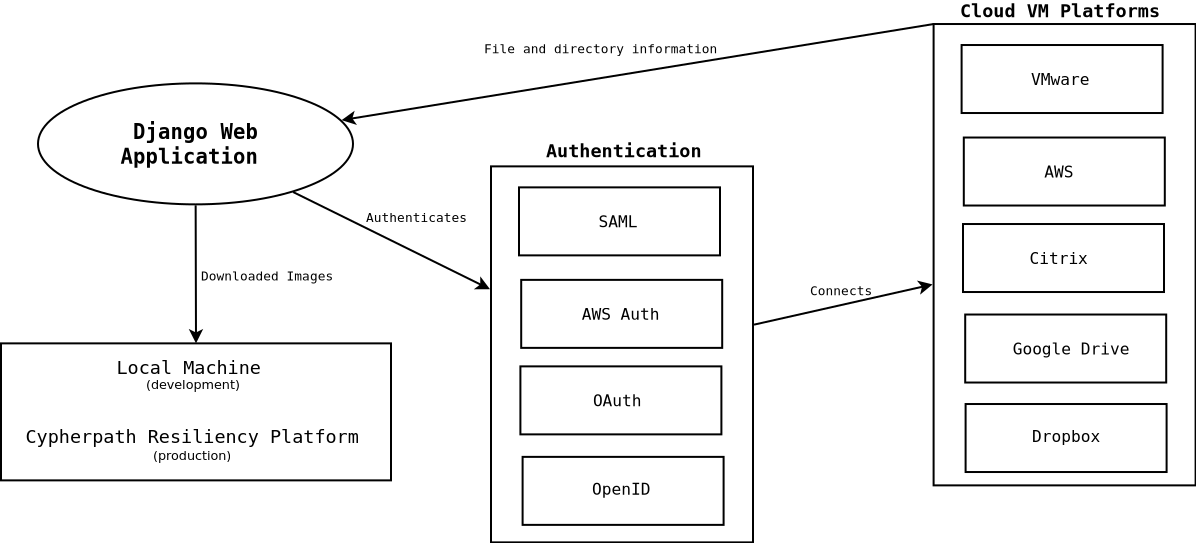
\includegraphics[scale=.4]{downloader_env}
        \caption{A visual representation of the applications environment.}
    \end{figure}


        \subsection{Web Application}
        The web server that serves the application will be Django's built in development server and when the project is completed, Cypherpath will integrate
        the web application into their existing ecosystem. The Django application will host the functionality of the application, including template for the 
        upload page, where users provide Virtual Machine URLs. Additionally the Django framework will allow the usage of python classes that will enable the 
        backend operation of the application.

        
        \subsection{Authentication API's}
        The application will authenticate to the cloud platforms with various authentication methods and API's. To start with, the application will need to support
        SAML and AWS Authentication, but will need to be designed in a modular fashion so that other authentication methods can be added later on such as OpenID and OAuth.
        The authentication would provide a token to verify the users for their Virtual Machines, the application will not provide previous states for the use of the 
        webiste, nor will it save previous Virtual machine URLS. The token will be passed to the request for access to the Virtual Machine URL provided



        \subsection{Cloud Storage API's}
        Once the application is authenticated to a Cloud Storage platform it will gather the directory structure for showing to the user and allowing them to select
        which of their files they would like to download. To start with the application will need to support interacting with VMware and Amazon Web Services. The API's
        that are neccessary for the communication, would request the Virtual Disk Image in which it will gather the necessary information to provide users the files they 
        would wish to interact with. The application will only interact with the Virtual Disk Image of the specified machines. The application will need to be designed so 
        that these interactions are modular to enable adding support for other cloud platforms later. Other cloud platforms that will be included, time permitting, are 
        Citrix, Google Drive and Dropbox.


        \subsection{Local Storage}
        Once the user has selected which files to download from their cloud platform, the application will download those
        files to the user's local storage. The user will not get the option to download specific files however. Unless time permitting
        allows implementation of the process. The Download will create copies of all user files from the Virtual disk to Local Memory, 
        The Local Storage location will not be able to be specified unless predefiened by the download protocol of the user. Nothing else 
        needs to be done with the files because after the application is finished and Cypherpath has integrated the web application into 
        their platform, they will direct the downloads where they need them.


    \section{Operation}
    In the following sections the operation of the application will be described, including starting the application
    (invocation), the commands the application uses and finally, how to close or terminate the application.

        \subsection{Invocation}
        Since the application will be integrated into Cypherpath's platform, the application will be started using Django's built-in development webserver and
        the user will not need to be authenticated to use the application. To invoke the application the user will simply enter the URL for the application.
        They will then be presented with the screen of the application. The Screen will have a single input text box for a user to insert a URL. Additionally 
        a submit button will be provided for them to continue to step through the application. 

        The user interface and Invocation of the machine are simple, to later be integrated into Cyperpaths resiliency tool, where the URL location will be dropped 
        and incorperated as a tool for their application. The main interface will remain the same by providing users with a single input option and a submission button.
        If there is an error in the initial URL provided the user will be prompted with an error that either the machine doesnt exist, or if invalid credentials 
        were provided, will be prompted as such.

        \subsection{User Actions}
            \subsubsection{Enter URL}
            The user can enter a URL that goes to their cloud platform (VMware or AWS initially). The text box will be centrally located with a design to help users clearly
            see where to input the URL, the box will also have shadow text requesting input. The application will figure out which cloud platform the URL belongs to, through a GET 
            request to the URL. If an error occurs with the GET request the user will be notified of the error. If the request is successful then the user will have to
            provide their login credentials, on a pop-up screen. The authentication will be verified with the platform they are using, (SAML for VMWare and AWS for AWS).
            Once authenticated the application will present the user with their files and folders that are on that platform.
            
            \subsubsection{Select URL} -- unsure of necessity for this
            In addition to the text box to enter a URL the user will also be presented with a list of previously entered URLs. The user will be able to remove URL's from this list, reconnect to them
            or close the session with that cloud platform.

            \subsubsection{Display File Structure}
            Once the user has selected a cloud platform and is authenticated, they will be presented with their directory structure on that platform. They will only see high level directories initially
            however will be able to open the directories to see files located within. They can use this information to verify all files were retrieved from the Virtual Disk. From here the user will be 
            provided the option to download the files locally. Unless specified differently in their browser download protocol, the user can expect to find copies of the files in their Download folder
            Cyperpath will later implement this to upload to their resiliency tool.

            \subsubsection{Download}
            The user will be provided with a interface that shows them the file structure of the Virtual Disk. A component of the display will be an optional download button. If the user wants to verify
            their files were downloaded properly the files will be neatly displayed to do so. Otherwise when the user is ready to download they will have to click the download button. The download itself 
            will default to their predetermined browser download location. The user will see total download completed, (This needs to be solved->) The user will be provided with a prompt to show how much
            the download has completed and the remaining time till completion.

            \subsubsection{Error Catching}
            Errors will be detected through the various aspects of the program. If the users provides an invalid URL, they will be prompted to provide a valid one. If the user does not provide valid credentials
            they will be prompted to provide proper ones. There will be no limit to the ammount of access atempts unless provided by the Authentication package provided by Python3. If provided then the max entry
            attempts will be set to 3 attempts as per standard. Additionally if there are any errors in a download, the user will be prompted and the download needing to be reatempted, however requirements specified
            provide that the download start over entirely. Unnecessary to keep track of progress and contine where left off previously before an error.

        \subsection{Termination}
        Since the user is not authenticated to the web application, to terminate their interaction with the application they will simply close the browser tab or window that has the
        application open. Use of the authentication token will be deleted as well per use, there will be no cookies to remember users everytime they log into the accounts. Upon Termination
        of the application the user will have to go through the same steps everytime they use the application.


    \section*{References}
    % Reference the project plan?
    % Possibly reference documentation to the various API's?

    \appendix
    \section{Appendix}
    % Sample files, if any?
    % Maybe a sketch of the general page layout?

\end{document}
